\scanpage{387}
\mspage{111}
% archive sheet number: 386
\figure{\makebox[\linewidth][l]{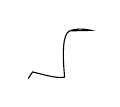
\begin{tikzpicture}[x=.55cm,y=.55cm]
\draw (0,0) -- (.1,.15) .. controls (.4,.08) and (.63,0) .. (.84,.03)
.. controls (.79,.57) and (.79,1.03) .. (.96,1.10)
.. controls (1.10,1.16) and (1.34,1.14) .. (1.45,1.11)
-- (.98,1.10);
\end{tikzpicture}}}
Reste l'axiome de \deleted{l'objet final}\inserted{contractibilité} : si $S$ dans $\mathrm{Cat}$ \deleted{a un objet final}\inserted{est \unsure{contractible|contractile}}, est-il $\mathrm{HOT}_W$-asphérique i.e. le foncteur
\[
\mathrm{HOT}_W(e)=\mathrm{Hot}_W\unsure{\relbar|\longrightarrow}\mathrm{HOT}_W(S)
\]
est-il pleinement fidèle ? Quand on dispose \deleted{de $\mathrm{Loc}(\unsure{3}$} de la théorie des $f_!$ ``\deleted{\unsure{dans}}\unsure{via|sur} $\mathrm{Cat}$'' (donc sous le seul axiome $\underline{\mathrm{Loc}(3\,\mathrm{bis})}$, on trouve ceci (noté dans $\underline{\overline{\mathrm{VI}}}$ p.~\unsure{202|252}) :
% slanted
\margin{moyennant $\mathrm{Loc}(3\,\mathrm{bis})$}

Soit $f:\unsure{\mathbb{S}|S}\to T$ une flèche de $\mathrm{Cat}$. Pour que ce soit une $\mathrm{HOT}_W$-équivalence, i.e. pour que $f^{\unsure{*|\wedge}}:\mathrm{HOT}_W(T)\to\mathrm{HOT}_W(S)$ induise un foncteur \uline{pleinement fidèle} sur la sous-catégorie des objets constants de $\mathrm{HOT}_W(T)$, il f. et s. que $\mathrm{hot}_W(f):\mathrm{hot}_W(S)\longrightarrow\mathrm{hot}_W(T)$ soit \unsure{iso.} Donc il \uline{suffit} que $f\in W$, et cette condition est aussi nécessaire si $\deleted{\unsure{g|S}}W$ est \deleted{fortement} saturé (axiome $\mathrm{Loc}(1\,\unsure{\mathrm{bis}|\mathrm{ter}})$).

Par acquit de conscience, j'explicite ici la démonstration. L'existence des foncteurs
